%% Technical Chapters

\chapter{System Overview}

The EvoRAG system is designed as a modular, privacy-preserving pipeline that enhances
traditional Retrieval-Augmented Generation by incorporating multi-agent reasoning,
evolutionary learning, and user-centric adaptation.

\section{Functional and Non-Functional Requirements}

\subsection{Functional Requirements}

\begin{itemize}

    \item \textbf{Real-Time Knowledge Ingestion:}
    The system shall fetch live article content at query time from NewsAPI, GNews,
    and a curated set of RSS feeds (BBC News, TechCrunch, Reuters) using the
    \texttt{requests} and \texttt{feedparser} libraries, triggered exclusively by
    the user's submitted query keyword — no pre-stored or pre-fetched corpus shall
    be used.

    \item \textbf{HTML Cleaning and Chunk Segmentation:}
    The system shall strip all non-content elements (CSS, JavaScript, navigation,
    advertisements) from fetched web pages using BeautifulSoup4, deduplicate articles
    by SHA-256 URL hashing, discard articles below a minimum character threshold,
    and segment retained content into overlapping chunks of 300--400 words with a
    50-word overlap to preserve cross-boundary context.

    \item \textbf{Vector Embedding and FAISS Indexing:}
    The system shall encode every text chunk into a dense vector using the
    \texttt{all-MiniLM-L6-v2} sentence-transformer model and persist all embeddings
    in a session-scoped local FAISS index alongside metadata (source URL, title,
    publication timestamp) to support semantic nearest-neighbour retrieval.

    \item \textbf{Contextual Chunk Retrieval:}
    The system shall, for each incoming user query, embed the query using the same
    \texttt{all-MiniLM-L6-v2} model and retrieve the top-3 semantically closest
    chunks from the FAISS index via approximate nearest-neighbour search, forming
    the grounding context for all subsequent persona generation calls.

    \item \textbf{Eight-Persona Parallel Response Generation:}
    The system shall invoke a locally hosted Ollama LLM (Llama~3.1 or Mistral~7B)
    once per query cycle with a structured prompt that instructs the model to
    generate eight independent analytical responses in a single call, each
    representing a distinct reasoning style: Analytical-Critical, Empirical-Evidential,
    Adversarial-Sceptical, Creative-Lateral, Domain-Expert, Temporal-Contextual,
    Risk-Evaluative, and Synthesis-Integrative.

    \item \textbf{Automated Peer-Review Scoring:}
    The system shall pass all eight persona drafts to the same local LLM in a
    second structured prompt, instructing it to act as an impartial judge and assign
    each response a score out of 30 across three dimensions — Factual Grounding (0--10),
    Analytical Depth (0--10), and Clarity (0--10) — returning results as a
    parseable JSON object.

    \item \textbf{Consensus-Based Answer Selection:}
    The system shall parse the judge's JSON score output, aggregate total scores per
    persona, select the persona with the highest aggregate score as the winner, and
    surface that response as the final answer together with the complete numerical
    score breakdown for all eight personas.

    \item \textbf{Source Attribution in Final Output:}
    The system shall append to every final answer the source URL, article title, and
    publication timestamp of each of the top-3 retrieved chunks that were used as
    the grounding context for that query cycle.

    \item \textbf{Evolutionary Win-Rate Tracking:}
    After every query cycle, the system shall update a local SQLite database with
    the winning persona's identifier, its total score, and any explicit user feedback
    signal (thumbs-up or thumbs-down), accumulating a longitudinal performance record
    per persona across all sessions.

    \item \textbf{Adaptive Persona Replacement:}
    The system shall compute a rolling win-rate for each persona from the SQLite
    history and, when a persona's win-rate falls below a configurable threshold,
    replace its prompt configuration with a newly generated variant without modifying
    the underlying Ollama model weights or restarting the backend service.

    \item \textbf{User Feedback and Voting Weight Adjustment:}
    The system shall record per-query user feedback via the React frontend and use
    accumulated feedback to adjust the relative voting weight assigned to each persona
    in the consensus scoring phase, such that personas consistently preferred by a
    specific user receive a weighted scoring advantage in future queries.

\end{itemize}

\subsection{Non-Functional Requirements}

\begin{itemize}

    \item \textbf{Local-Only Execution:}
    Every component of EvoRAG — including the Ollama LLM runtime, FAISS vector index,
    SQLite persona database, FastAPI backend, and React frontend — shall run entirely
    on the user's local machine. The system shall make no outbound network calls during
    the generation, scoring, or evolutionary update phases; network access is permitted
    only during the initial knowledge acquisition phase (NewsAPI, GNews, RSS).

    \item \textbf{Retrieval-Grounded Generation:}
    The LLM prompt issued for persona generation shall always include the top-3
    retrieved FAISS chunks as mandatory context. The system shall not issue any
    generation call without valid retrieval context; if the FAISS index returns zero
    results, the pipeline shall terminate early and return a structured
    ``no relevant context'' message rather than invoking the LLM on an empty context.

    \item \textbf{End-to-End Response Latency:}
    On the minimum hardware configuration (CPU-only inference with Llama~3.1 8B or
    Mistral~7B via Ollama), the complete pipeline — fetch, embed, retrieve, generate
    eight personas, score, and select — shall complete within 90 seconds per query.
    On the recommended configuration (NVIDIA RTX 3060 or equivalent with CUDA-enabled
    Ollama), this target reduces to 25 seconds per query.

    \item \textbf{FAISS Index Capacity and Retrieval Consistency:}
    The FAISS flat-L2 index shall handle a per-session knowledge base of up to
    10,000 text chunks (approximately 50--100 fully processed articles) with no
    measurable increase in nearest-neighbour search latency, as FAISS flat indices
    perform exact search in O(n) time over the embedding dimension, providing
    deterministic retrieval results for identical query embeddings.

    \item \textbf{Graceful Handling of News API Failures:}
    If NewsAPI or GNews returns a non-200 HTTP status or a response with zero
    articles, the pipeline shall automatically fall back to the configured RSS feed
    set and proceed with whatever content is available. If all three sources yield
    no usable content, the system shall return a structured failure response; it
    shall not raise an unhandled exception or crash the FastAPI server process.

    \item \textbf{Persona Score Transparency:}
    The React frontend shall display the full scoring table — all eight persona names,
    their individual Factual Grounding, Analytical Depth, and Clarity scores, and
    aggregate totals — alongside the winning response for every completed query.
    This display shall not be optional or hidden behind additional user interaction.

    \item \textbf{SQLite Schema Stability Across Sessions:}
    The evolutionary tracking database (SQLite) shall persist across server restarts.
    The schema (persona identifier, win count, total queries, last updated timestamp,
    user feedback score) shall not be modified between sessions; accumulated win-rate
    history shall carry forward and inform persona replacement decisions continuously.

\end{itemize}

\section{Software Requirements}

The EvoRAG system relies entirely on software-based components and locally hosted
models, enabling full execution without cloud dependencies or external API calls.
Table~\ref{tab:software} summarises the complete software environment.

\vspace{0.5em}

\begin{center}
\small
\renewcommand{\arraystretch}{1.5}
\begin{longtable}{|p{3.8cm}|p{3.5cm}|p{6.2cm}|}
\caption{Software Requirements}
\label{tab:software} \\
\hline
\textbf{Component} & \textbf{Specification} & \textbf{Purpose} \\
\hline
\endfirsthead
\hline
\textbf{Component} & \textbf{Specification} & \textbf{Purpose} \\
\hline
\endhead
\hline
\endfoot
Programming Language & Python 3.11+ &
Extensive ML ecosystem, cross-platform compatibility, and asynchronous
programming support for the multi-persona generation pipeline. \\
\hline
Embedding Library & sentence-transformers $\geq$ 3.1.0 &
Converts text chunks into high-dimensional vector representations for
semantic retrieval using the all-MiniLM-L6-v2 model. \\
\hline
Vector Search Library & faiss-cpu $\geq$ 1.9.0 &
Provides efficient vector indexing and approximate nearest-neighbour
lookup for the retrieval pipeline. \\
\hline
Numerical Computing & numpy $\geq$ 1.26 &
Enables efficient array operations and mathematical computations
throughout the pipeline. \\
\hline
Web Framework & fastapi $\geq$ 0.115.0 &
Exposes the EvoRAG pipeline as a RESTful backend API with automatic
OpenAPI documentation. \\
\hline
ASGI Server & uvicorn[standard] $\geq$ 0.30.0 &
Serves the FastAPI application with support for asynchronous request
handling and HTTP/2. \\
\hline
HTTP Client & httpx $\geq$ 0.27.0 &
Handles asynchronous inter-service communication within the pipeline. \\
\hline
Feed Parser & feedparser $\geq$ 6.0.11 &
Parses RSS and Atom feeds during the knowledge acquisition phase. \\
\hline
HTML Parser & beautifulsoup4 $\geq$ 4.12.3 &
Cleans and extracts textual content from fetched web articles. \\
\hline
HTTP Library & requests $\geq$ 2.32.0 &
Supports synchronous web requests during the data fetching phase. \\
\hline
Environment Manager & python-dotenv $\geq$ 1.0.1 &
Manages environment variables and configuration securely at runtime. \\
\hline
Local LLM Runtime & Ollama $\geq$ 0.3.0 with Llama~3.1~(8B) / Mistral~7B &
Hosts and serves open-source large language models entirely on local
hardware, eliminating any third-party API dependency. \\
\hline
Embedding Model & nomic-embed-text (via Ollama) &
Provides a locally hosted text embedding model as an alternative to
sentence-transformers for fully offline operation. \\
\hline
Vector Store & FAISS (local, in-process) &
Persists and queries embedded knowledge chunks with no external
database server required. \\
\hline
Database & SQLite 3 (built-in) &
Stores persona performance metrics, win rates, and evolutionary
history in a lightweight, file-based local database. \\
\hline
Frontend & React.js $\geq$ 18.0 &
Provides real-time query input, persona draft display, voting breakdown
visualisation, and user feedback controls. \\
\hline
Operating System & Windows 10/11 or Ubuntu 22.04+ &
Required to support the Python 3.11+ runtime and the Ollama local
model serving platform. \\
\hline
Development Environment & Visual Studio Code $\geq$ 1.89 &
Offers integrated debugging, code completion, and version control
capabilities. \\
\hline
\end{longtable}
\end{center}

\clearpage



\section{Hardware Requirements}

The EvoRAG system runs entirely on a single local development workstation and does
not require specialised server infrastructure or cloud hardware.
Table~\ref{tab:hardware} summarises the minimum and recommended hardware configuration.

\vspace{0.5em}

\begin{table}[H]
\centering
\caption{Hardware Requirements}
\label{tab:hardware}
\renewcommand{\arraystretch}{1.5}
\footnotesize
\begin{tabularx}{\linewidth}{|p{2.2cm}|X|X|X|}
\hline
\textbf{Component} & \textbf{Minimum} & \textbf{Recommended} & \textbf{Justification} \\
\hline
Processor &
Intel Core i5 (8th Gen) / AMD Ryzen 5 3600 &
Intel Core i7 (12th Gen) / AMD Ryzen 7 5800X &
Required for local LLM inference and concurrent multi-persona generation. \\
\hline
RAM &
16 GB DDR4 &
32 GB DDR4/DDR5 &
Supports simultaneous execution of Ollama LLM, FAISS search, FastAPI backend, and React frontend. \\
\hline
GPU &
NVIDIA GTX 1660 (6 GB VRAM) or CPU-only &
NVIDIA RTX 3060 (12 GB VRAM) or RTX 4070 &
Accelerates LLM inference via CUDA; system runs on CPU by default but GPU reduces latency significantly. \\
\hline
Storage &
20 GB SSD &
50 GB NVMe SSD &
Accommodates LLM weights (4--8 GB), FAISS index, SQLite database, and fetched knowledge articles. \\
\hline
Operating System &
Windows 10 (64-bit) or Ubuntu 20.04 LTS &
Windows 11 or Ubuntu 22.04 LTS &
Required for Python 3.11+ runtime and Ollama local model serving platform. \\
\hline
Network &
\multicolumn{2}{X|}{Broadband internet (knowledge acquisition phase only)} &
Required only during initial fetch via NewsAPI/GNews/RSS; all inference and retrieval run fully offline. \\
\hline
\end{tabularx}
\end{table}

\section{System Architecture}

The EvoRAG architecture is structured as a continuous, evolutionary loop consisting of ten primary stages. This architecture ensures that the system not only provides grounded answers but also improves its analytical capabilities over time based on performance metrics and user feedback.

The workflow follows these stages:

\begin{enumerate}
    \item \textbf{User Query:} The process begins when a user submits a question to the system.
    
    \item \textbf{Data Retrieval:} Relevant documents and raw data are fetched from various APIs and external sources.
    
    \item \textbf{Processing \& Embedding:} The retrieved data is cleaned, segmented into chunks, and converted into high-dimensional vector embeddings.
    
    \item \textbf{Vector Search:} The system searches the vector database to retrieve the most contextually relevant chunks for the specific query.
    
    \item \textbf{Multi-Persona Generation:} Responses are generated in parallel by multiple distinct AI personas (e.g., Analyst, Critic, Creative).
    
    \item \textbf{Consensus Voting:} The personas evaluate each other’s responses, scoring them based on quality, factual accuracy, and depth.
    
    \item \textbf{Final Answer:} The highest-scoring response is selected and delivered as the final output to the user.
    
    \item \textbf{User Feedback:} The user provides qualitative feedback (likes or dislikes), which is recorded by the system.
    
    \item \textbf{Performance Tracking:} The system tracks persona accuracy and scores, storing these performance metrics in a local database.
    
    \item \textbf{Evolutionary Update:} Based on performance trends, weak personas are replaced or refined, allowing the system to improve autonomously over time.
\end{enumerate}

\begin{figure}[H]
    \centering
    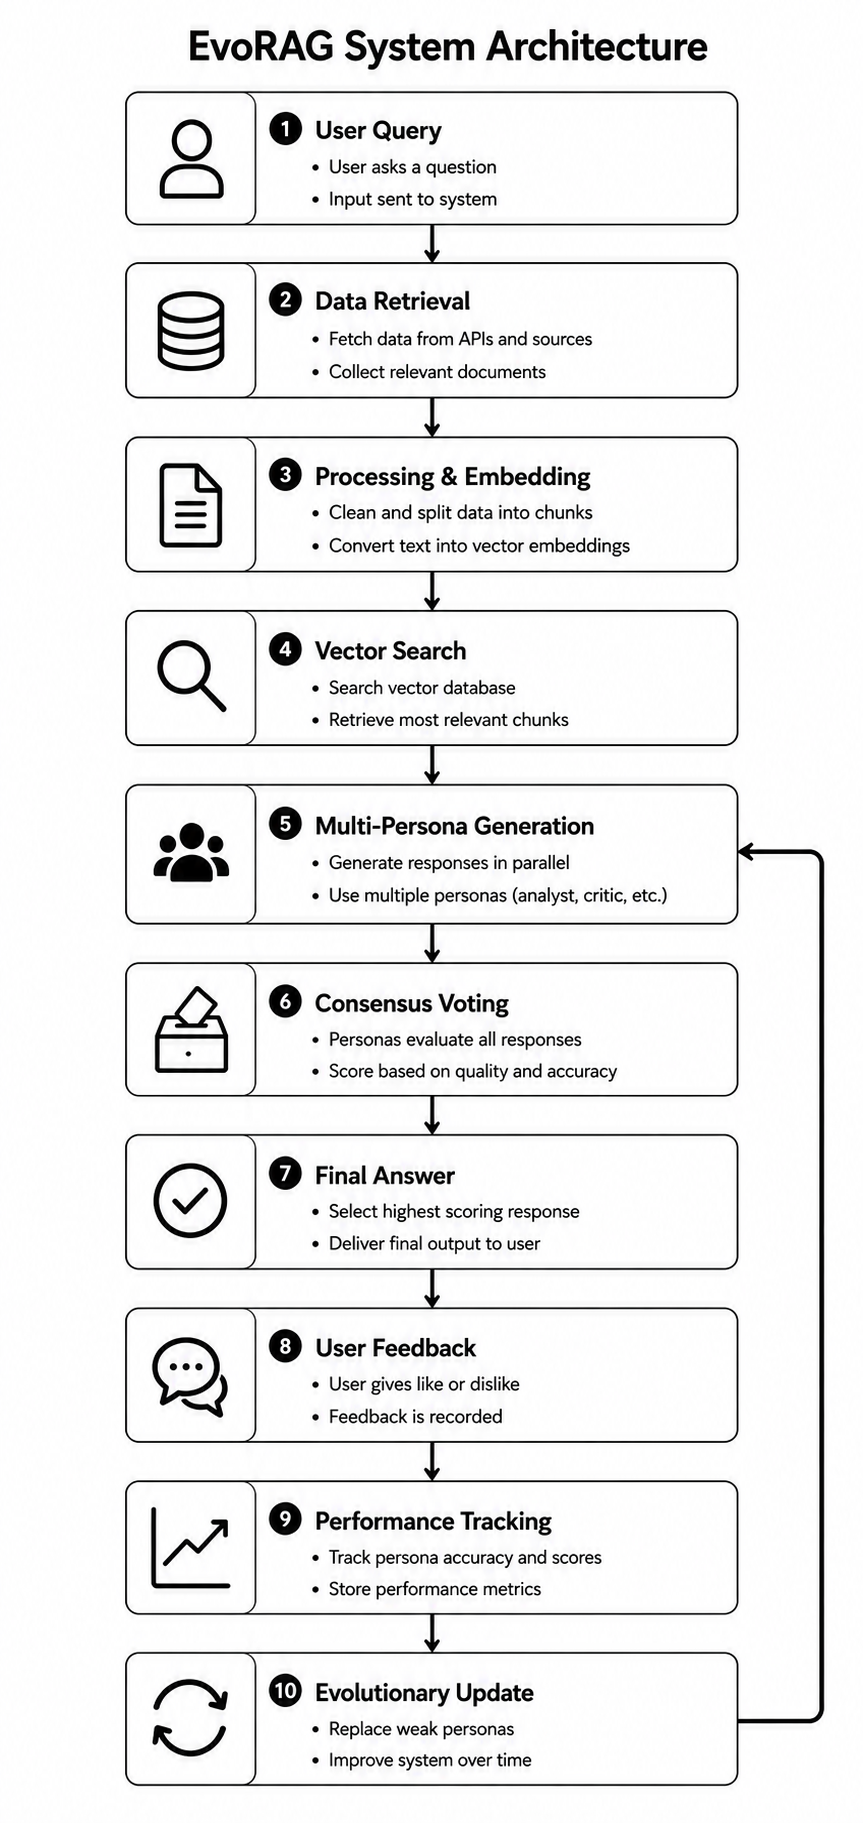
\includegraphics[width=0.70\linewidth]{Sys.png}
    \caption{EvoRAG System Architecture FlowChart}
    \label{fig:evorag_architecture}
\end{figure}

\begin{figure}[H]
    \centering
    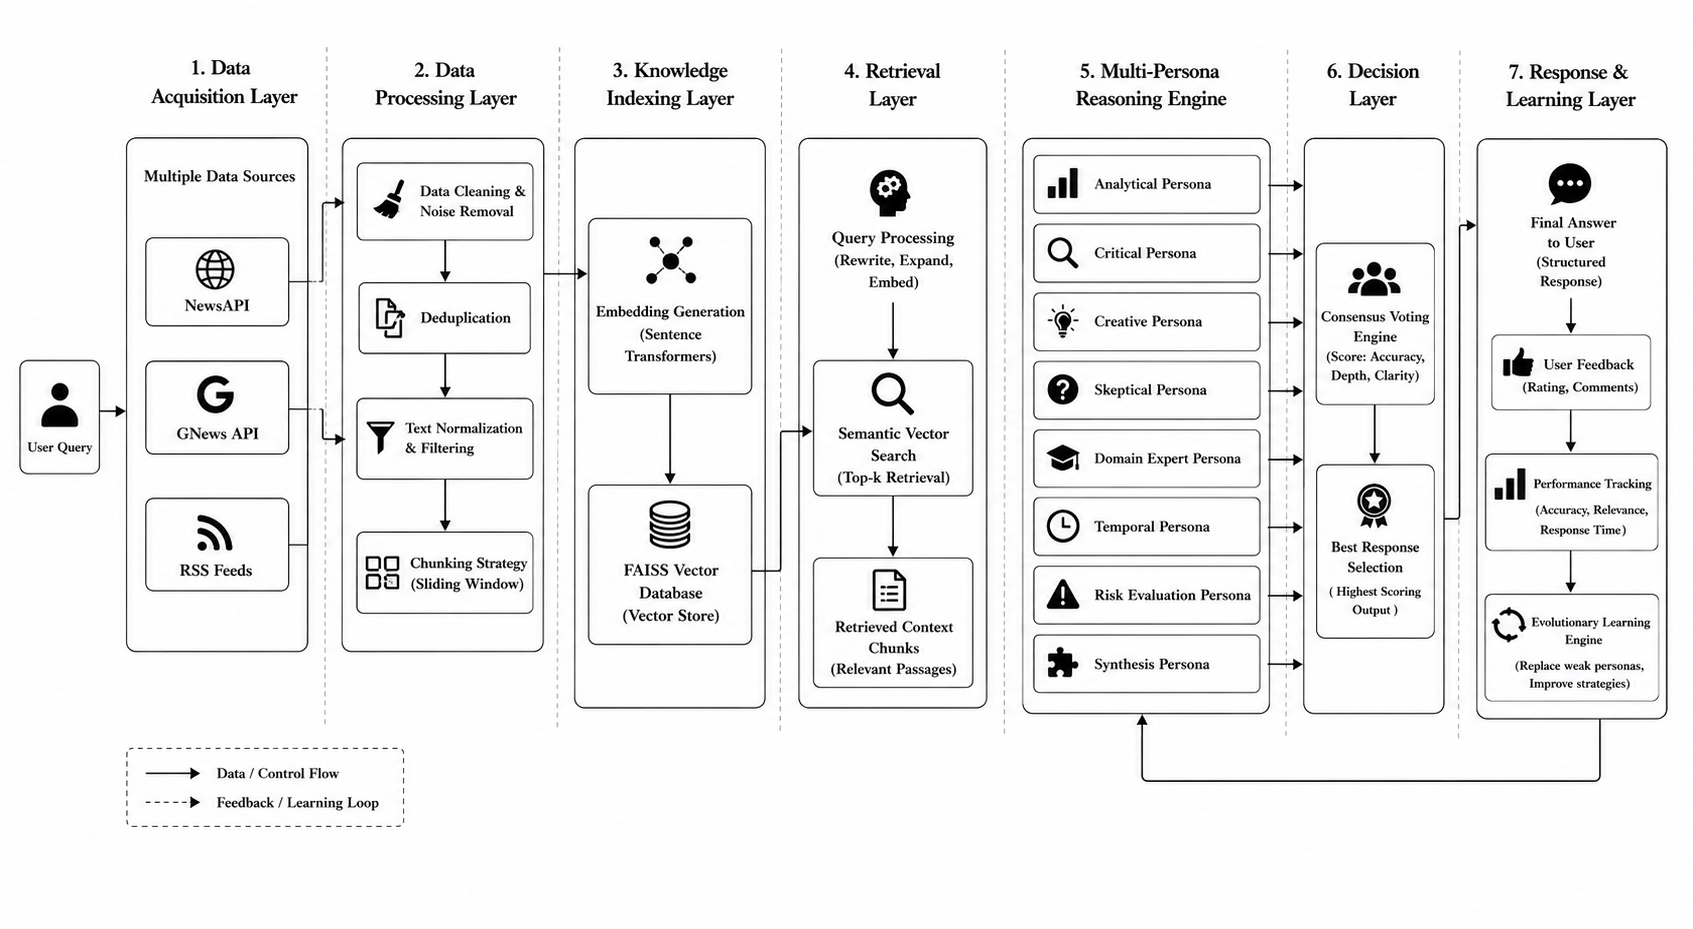
\includegraphics[width=0.95\linewidth]{sA2.png}
    \caption{EvoRAG System Architecture and Evolutionary Loop}
    \label{fig:evorag_architecture}
\end{figure}


\subsection{High Level Design}

The high level design illustrates the major modules of the EvoRAG system and their interactions.

\begin{figure}[H]
    \centering
    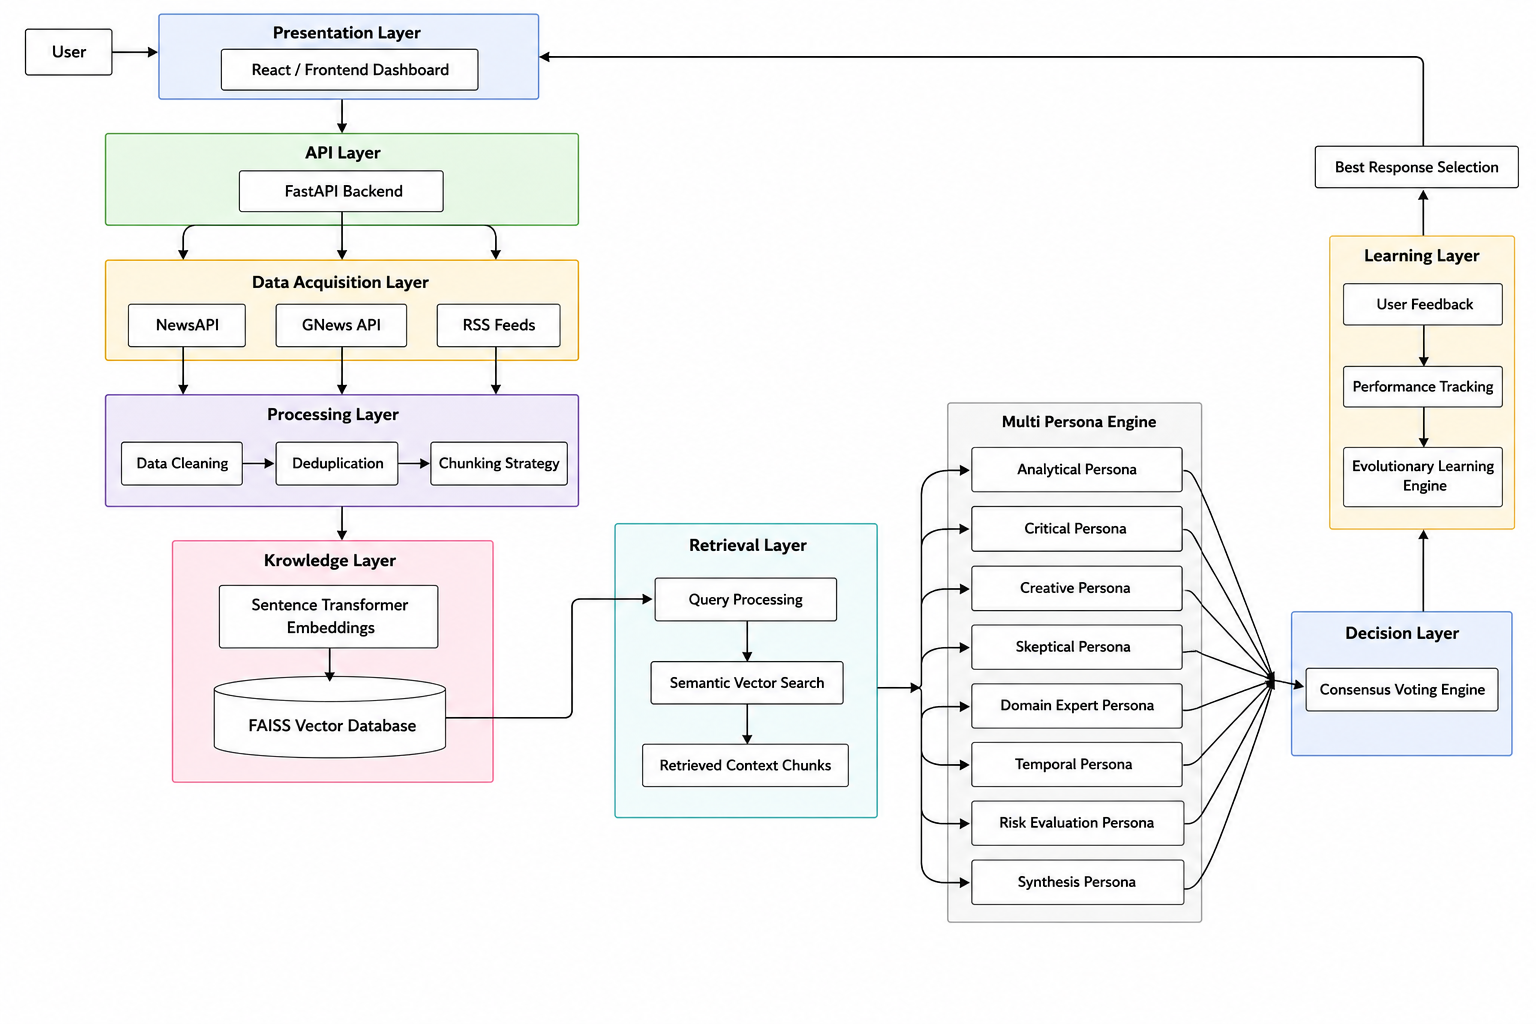
\includegraphics[width=0.85\linewidth,height=0.85\textheight,keepaspectratio]{hld.png}
    \caption{EvoRAG High Level Design}
    \label{fig:hld}
\end{figure}

\clearpage

\subsection{Low Level Design}

The low level design provides a detailed view of the internal logic within each
module, specifying the data flows, component interactions, API contracts, and
the sequence of operations that occur during a complete query-to-response cycle,
including the evolutionary feedback loop.

\begin{figure}[H]
    \centering
    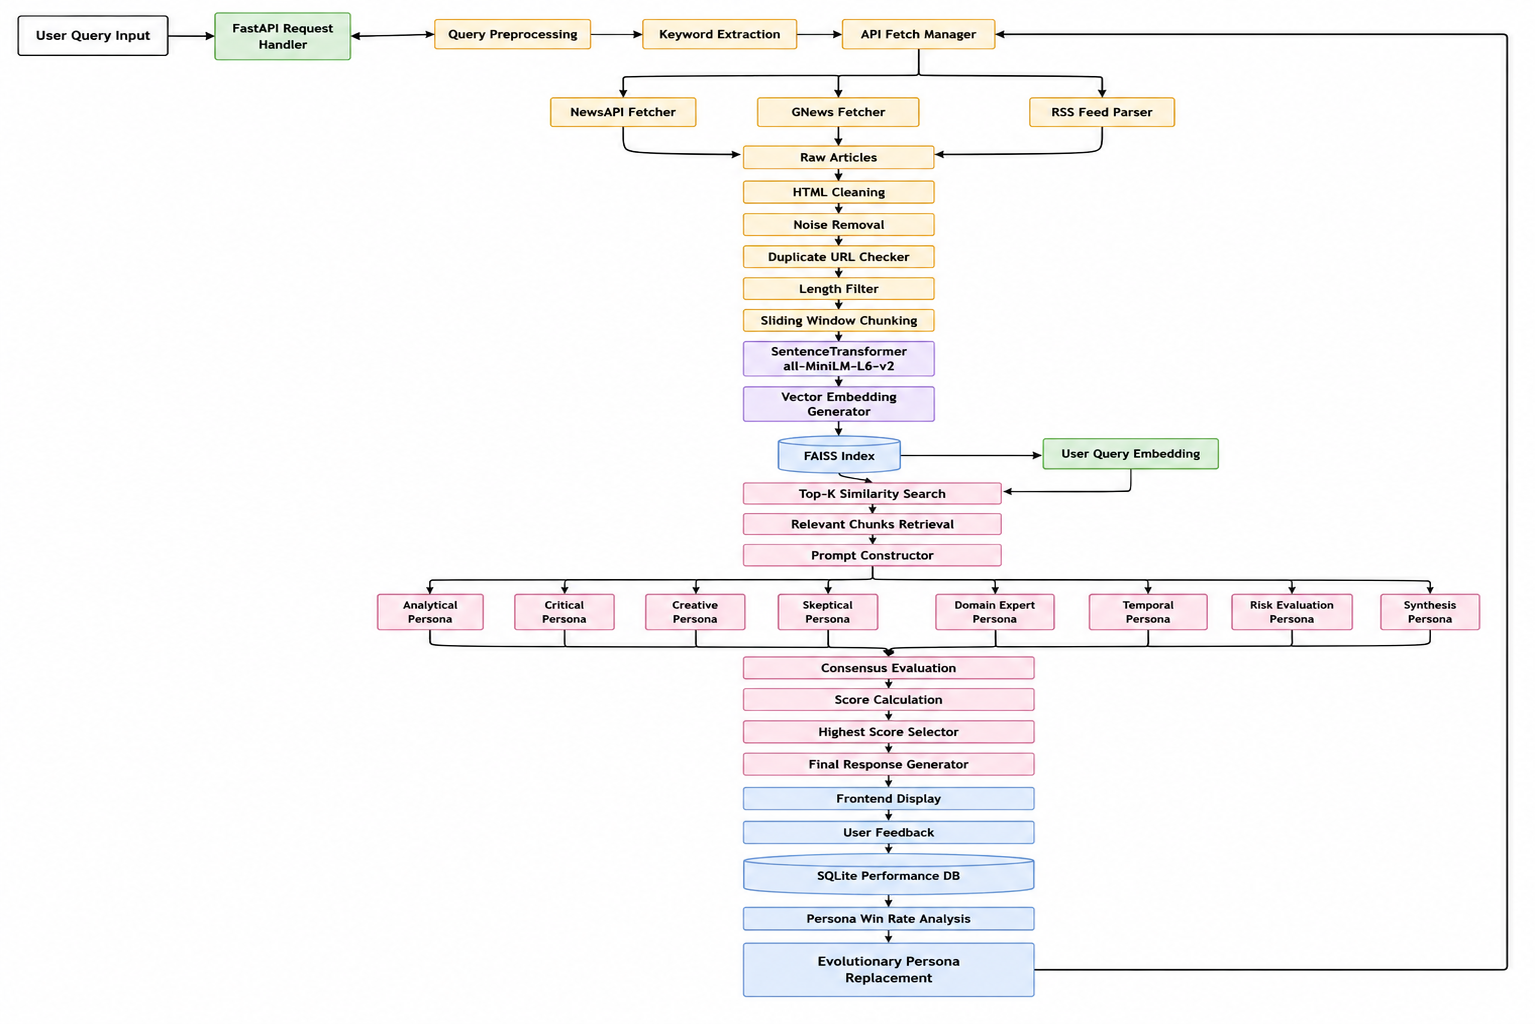
\includegraphics[width=\linewidth,height=\textheight,keepaspectratio]{lld2.png}
    \caption{EvoRAG Low Level Design}
    \label{fig:lld}
\end{figure}}

\chapter{Methodology}

\begin{figure}[H]
    \centering
    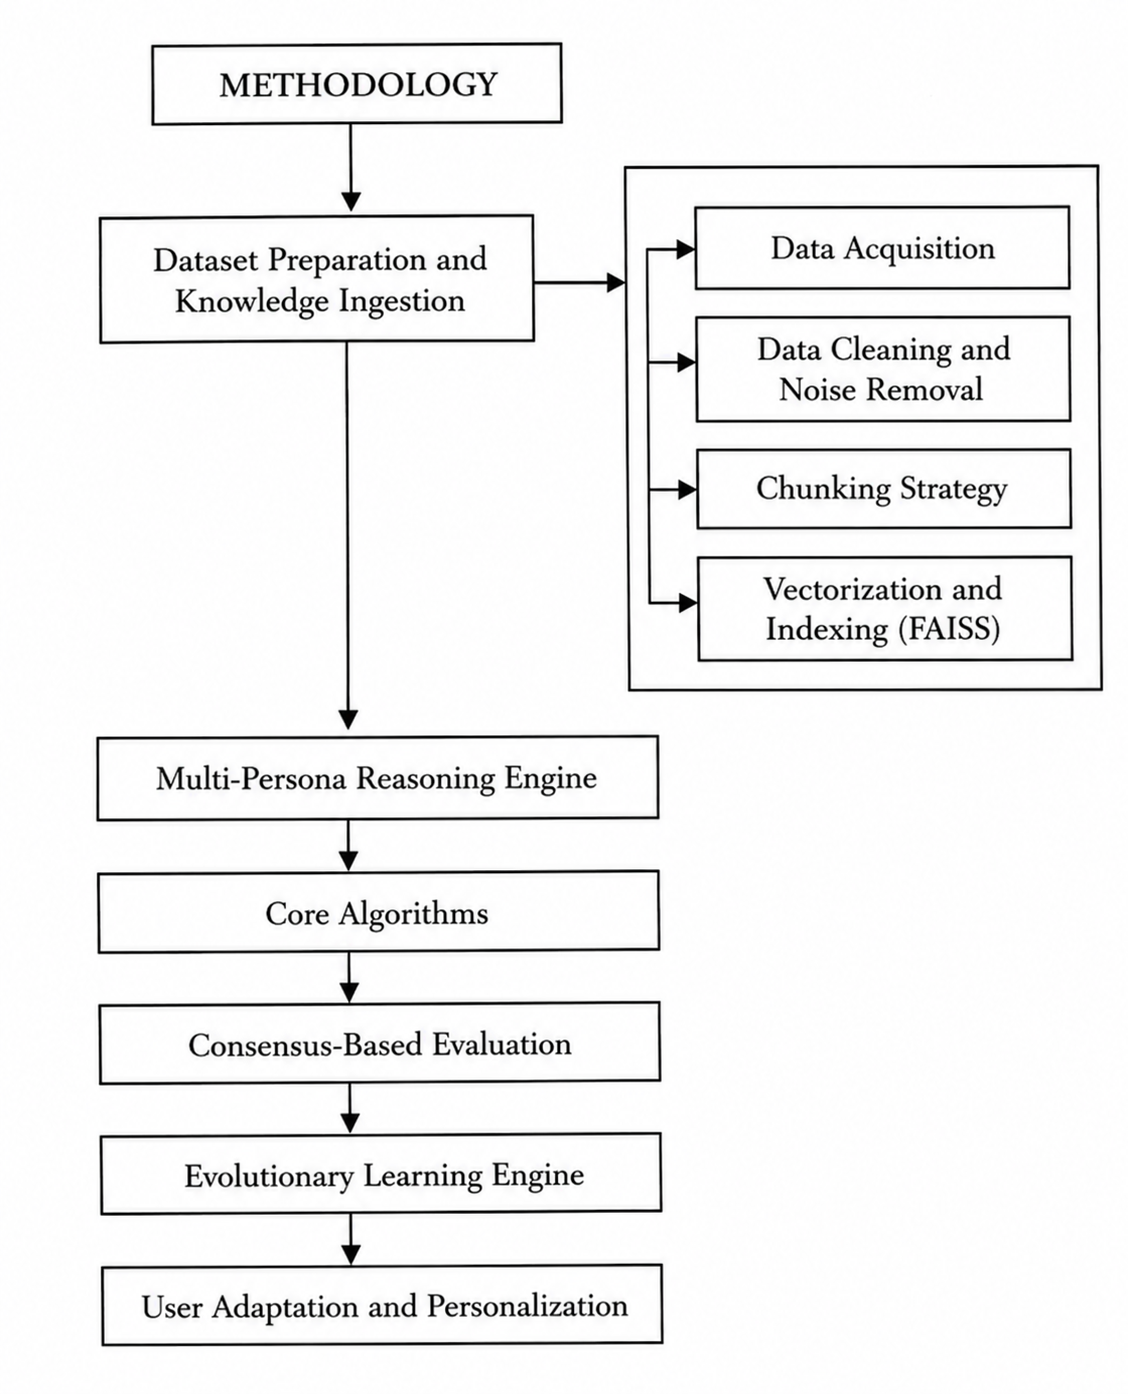
\includegraphics[width=0.75\linewidth]{method.png}
    \caption{EvoRAG Methodology Flowchart}
    \label{fig:method_flowchart}
\end{figure}

Figure~\ref{fig:method_flowchart} illustrates the complete EvoRAG methodology flow. The methodology of EvoRAG is divided into four core engines that work in tandem to produce high-quality, personalized results. It begins with dynamic data acquisition, progresses through data cleaning and chunking, indexes the resulting semantic vectors, and finishes with parallel multi-persona reasoning evaluated through consensus.

\section{Implementation}

This section explains the key implementation steps in the EvoRAG pipeline, covering data acquisition, cleaning, removal, chunking, indexing, and multi-persona reasoning.

\subsection{Data Acquisition}

The pipeline aggregates textual knowledge from three distinct live sources:

\begin{itemize}
    \item \textbf{NewsAPI:} Fetches comprehensive, real-time news articles from thousands of global publishers based on the user’s query keyword.
    \item \textbf{GNews API:} Retrieves top-ranking, highly credible articles indexed by Google News, providing broad topical coverage.
    \item \textbf{RSS Feeds:} Continuously monitored feeds from trusted, high-quality domains (e.g., BBC News, TechCrunch, Reuters) ensure a reliable baseline of verified journalism.
\end{itemize}

HTTP requests are handled via the \texttt{requests} library, while \texttt{feedparser} is used specifically for structured RSS feed parsing.

\subsection{Data Cleaning and Noise Removal}

Raw web content contains significant noise that must be eliminated before the data can be used for reasoning. The following cleaning steps are applied automatically:

\begin{itemize}
    \item \textbf{HTML Stripping:} The BeautifulSoup4 library parses each fetched page and removes all non-content elements including CSS stylesheets, JavaScript blocks, navigation menus, and advertisement banners, isolating only the pure article body text.
    \item \textbf{Deduplication:} Each article URL is hashed using SHA-256 before ingestion. Any URL whose hash already exists in the current session index is silently discarded, preventing the LLM from processing redundant or repeated information.
    \item \textbf{Length Filtering:} Articles falling below a minimum character threshold are discarded as they are unlikely to contain substantive analytical content.
\end{itemize}

\subsection{Chunking Strategy}

Large Language Models operate under strict context window and token limitations, making it impractical to feed entire articles as input. To address this, a sliding-window chunking strategy is applied.

\begin{itemize}
    \item \textbf{Chunk Size:} Each cleaned article is split into segments of approximately 300--400 words.
    \item \textbf{Overlap:} A 50-word overlap is maintained between consecutive chunks to ensure that contextual continuity across paragraph boundaries is preserved and no critical information is lost at chunk edges.
\end{itemize}

\subsection{Vectorization and Indexing (FAISS)}

Once chunked, the text segments are transformed into a machine-searchable vector database.

\begin{itemize}
    \item \textbf{Embedding Generation:} Each text chunk is passed through the \texttt{sentence-transformers} model (\texttt{all-MiniLM-L6-v2}), which encodes it into a high-dimensional dense vector representation capturing its semantic meaning.
    \item \textbf{FAISS Indexing:} All generated embeddings are stored in a local FAISS (Facebook AI Similarity Search) index using a flat L2 index structure that performs exact nearest-neighbour search, guaranteeing deterministic retrieval for identical query embeddings across sessions.
    \item \textbf{Metadata Preservation:} Alongside each embedding, the source URL, article title, and publication timestamp are stored as metadata to support source attribution in the final output.
\end{itemize}

This FAISS index constitutes the runtime dataset from which the multi-persona generation engine retrieves its grounding context.
At query time, the user's input is independently embedded using the same \texttt{all-MiniLM-L6-v2} model to produce a query vector, which is then compared against all stored chunk vectors to return the top-3 most semantically relevant passages as the retrieval context.
\subsection{Multi-Persona Reasoning Engine}

Instead of relying on a single output, EvoRAG employs a parallel generation strategy that produces eight independent analytical responses within a single LLM call.

\begin{itemize}
    \item \textbf{Structured Single-Call Generation:} The retrieved context and user query are packaged into a structured prompt that instructs the locally hosted Ollama LLM to simultaneously produce eight distinct persona responses in a single inference call, formatted as a parseable JSON object.
    \item \textbf{Diverse Personas:} Eight analytical personas — Analytical-Critical, Empirical-Evidential, Adversarial-Sceptical, Creative-Lateral, Domain-Expert, Temporal-Contextual, Risk-Evaluative, and Synthesis-Integrative — each produce an independent perspective grounded in the same retrieved context.
    \item \textbf{JSON Parsing and Validation:} The raw LLM output is parsed as a structured JSON object; each entry contains the persona name and its corresponding answer text, which are then passed directly to the peer-review scoring stage.
    \item \textbf{Goal:} To improve reasoning depth and eliminate the single-perspective bias inherent in standard RAG models, while maintaining full local execution without multiple sequential API calls.
\end{itemize}

\clearpage

\section{Core Algorithms}

The technical implementation of EvoRAG relies on several core algorithmic concepts,
with the primary orchestration handled by the EvoRAG Pipeline described below.

\subsubsection{Evolutionary Multi-Persona RAG Algorithm}

\vspace{0.5em}

\begin{algorithm}[H]
\caption{EvoRAG Pipeline --- Query to Consensus Response}
\small
\SetAlgoLined
\KwIn{$user\_query$}
\KwOut{$best\_persona,\ best\_answer,\ score\_breakdown,\ sources$}

\BlankLine
\tcp{Step 1: Retrieval}
$chunks \leftarrow \text{FAISS\_Retrieve}(user\_query,\ top\_k=3)$\;
\If{$chunks = \emptyset$}{
    \Return \textit{``No relevant context found.''}\;
}
$context \leftarrow \text{Merge}(chunks)$\;

\BlankLine
\tcp{Step 2: Multi-Persona Generation}
$personas \leftarrow \{$Analytical-Critical, Empirical-Evidential, Adversarial-Sceptical,
Creative-Lateral, Domain-Expert, Temporal-Contextual, Risk-Evaluative, Synthesis-Integrative$\}$\;
$prompt_{gen} \leftarrow \text{BuildPrompt}(user\_query,\ context,\ personas)$\;
$drafts \leftarrow \text{ParseJSON}(\text{LLM}(prompt_{gen}))$\;

\BlankLine
\tcp{Step 3: Peer-Review Scoring}
$prompt_{judge} \leftarrow \text{BuildJudgePrompt}(user\_query,\ drafts)$\;
$scores \leftarrow \text{ParseJSON}(\text{LLM}(prompt_{judge}))$\;
\tcp*[r]{Factual Grounding (0--10) + Analytical Depth (0--10) + Clarity (0--10) $= /30$}

\BlankLine
\tcp{Step 4: Consensus Selection}
$best\_persona \leftarrow \arg\max_{p \in personas}\ scores[p]$\;
$best\_answer \leftarrow drafts[best\_persona].answer$\;

\BlankLine
\tcp{Step 5: Output}
\Return $\{best\_persona,\ best\_answer,\ scores,\ chunks.metadata\}$\;
\end{algorithm}

\section{Consensus-Based Evaluation}

The system implements a self-regulating peer-review mechanism.

\begin{itemize}
    \item \textbf{Peer Voting Mechanism:} Each persona evaluates all generated responses, acting as a “judge” for others.
    
    \item \textbf{Scoring Criteria:} Responses are graded on three dimensions: Factual Grounding, Analytical Depth, and Clarity.
    
    \item \textbf{Final Selection:} The highest-scoring response, representing the consensus of the brainstorming session, is chosen as the final output.
\end{itemize}

\section{Evolutionary Learning Engine}

To ensure continuous improvement without retraining the base LLM, an evolutionary layer is added.

\begin{itemize}
    \item \textbf{Performance Tracking:} The win rates and qualitative scores of each persona are stored in a local SQLite database.
    
    \item \textbf{Adaptive Replacement:} Personas that consistently fail to win the peer-review or receive poor user feedback are periodically replaced with new persona variants.
    
    \item \textbf{Self-Improvement:} This allows the system to evolve its intellectual makeup over time based on the specific types of queries it receives.
\end{itemize}

\section{User Adaptation and Personalization}

The system adapts to individual user needs through a feedback loop.

\begin{itemize}
    \item \textbf{Feedback Integration:} The UI records user likes and dislikes for each response.
    
    \item \textbf{Affinity Modeling:} Personalized preference profiles are built, identifying which personas or response styles the user prefers.
    
    \item \textbf{Adaptive Output:} The voting weights in the consensus phase are dynamically adjusted based on these preference profiles.
\end{itemize}